%----------------------------------------------------------------------------------------
%	PACKAGES AND THEMES
%----------------------------------------------------------------------------------------
\documentclass[aspectratio=169,xcolor=dvipsnames]{beamer}
\usetheme{Simple}

\usepackage{hyperref}
\hypersetup{
    colorlinks,
    linkcolor=black, % Overview
    urlcolor=blue    % \href#2
}

\usepackage{graphicx} % Allows including images

%----------------------------------------------------------------------------------------
%	Macros
%----------------------------------------------------------------------------------------
\newcommand{\bi}{\begin{itemize}}
\newcommand{\ei}{\end{itemize}}
\newcommand{\param}[1]{{$\langle#1\rangle$}}
\def\figs{figs2}
%----------------------------------------------------------------------------------------
%	TITLE PAGE
%----------------------------------------------------------------------------------------

% The title
\title[short title]{FAIR Data}
\author{
\includegraphics[scale=0.5]{ildg-logo}\\Working Groups}
\institute{Hands-on Workshop}
\date{June 14, 2023 } % Date, can be changed to a custom date


%----------------------------------------------------------------------------------------
%	PRESENTATION SLIDES
%----------------------------------------------------------------------------------------
\begin{document}

\begin{frame}
    % Print the title page as the first slide
    \titlepage

\end{frame}

\begin{frame}{Overview}
    % Throughout your presentation, if you choose to use \section{} and \subsection{} commands, these will automatically be printed on this slide as an overview of your presentation
    \tableofcontents
\end{frame}

%----------------------------------------------------------------------------------------
%================================================
\section{Lattice Data goes FAIR}
%================================================
\begin{frame}{FAIR Principles} 

  \hspace*{7em}
  \parbox{40mm}{
  \alert{F}indable\\
  \hspace*{3em} \alert{A}ccessible \\
  \hspace*{6em} \alert{I}nteroperable \\
  \hspace*{9em} \alert{R}eusable
  }
  \hfill
  \parbox{26mm}{\footnotesize
    \href{https://www.force11.orf}{force11.org}\\[-1mm]
    \hspace*{8mm}{\footnotesize $\vdots$}\\[-1mm]
    \href{https://www.nature.com/articles/sdata201618}{Wilkinson~2016}\\[-1mm]
    \hspace*{8mm}{\footnotesize $\vdots$}\\[-1mm]
    \href{https://www.go-fair.org/fair-principles}{go-fair.org}
  }

  \vspace*{5mm}
  \begin{itemize}
    \item It is becoming a mandatory \alert{requirement} by funding agencies \\
      {\small ``The [European] Commission will work with global policy and research
        partners to foster cooperation and to create a level playing field in
        scientific data sharing and data-driven science.''\\
      \hfill\href{https://eur-lex.europa.eu/legal-content/en/TXT/?uri=CELEX:52016DC0178}{EU Commission, COM(2016)178}
      }
    \item provides \alert{guiding principles}, not an implementation
    \item conceptually refers to three types of entities: %%% FAIR-go
      \begin{itemize}
        \item data = any digital object
        \item metadata (MD) = information about digital object
        \item infrastructure
      \end{itemize}
    \item requires machine actionable (meta)data
  \end{itemize}
\end{frame}

%------------------------------------------------
\begin{frame}{What does ``findable'' mean?}
  %% list requirements from Go Fair: https://www.go-fair.org/fair-principles/ [www.go-fair.org]) xxx}
  \begin{alertblock}{Findable}
    \begin{itemize}
      \item[F1] globally unique and persistent ID assigned to (M)D
      \item[F2] data described with rich MD %%% (see R1) % DP: drop
      \item[F3] MD includes data ID of data
      \item[F4] (M)D registered or indexed in a searchable resource
    \end{itemize}
  \end{alertblock}

  Metadata includes information on
  \begin{itemize}
  \item content (general and domain-specific vocabulary)
  \item provenance (who, when, where, how?)
  \item access (format, path, license, \ldots)
  \item \ldots
  \end{itemize}

\end{frame}
%------------------------------------------------
\newcommand{\access}[1]{
\begin{frame}{How does ILDG address ``findable''?}
  \begin{columns}[c] 
    \column{0.5\textwidth}
    Metadata
    \begin{itemize}
    \item follows a well-defined and rich schema
    \item stored \alert{separately} from data (big)
    \item searchable in central catalog of \alert{each} RG
    \end{itemize}
    
    \column{0.5\textwidth}
    \hspace*{-3mm}
    \includegraphics[height=35mm]{\figs/#1}
  \end{columns}
\end{frame}
}
\access{ildg-access1schema}
\access{ildg-access2}
%------------------------------------------------
\begin{frame}{Unique identifiers}

    \begin{columns}[c] 
      \column{0.70\textwidth}
      \begin{itemize}
      \item \alert{Ensembles:} have only MD (content, access permissions, \ldots)\\
        \hspace*{5em} {\tt \alert{mc}://\param{rg}/\param{collab}/\param{proj}/...} 
      \item Configurations: MD (related ensemble, provenance info)\\
        {\bf and} actual data\\
        \hspace*{5em} {\tt lfn://\param{rg}/\param{collab}/\param{proj}/...} 
      \end{itemize}

      \column{0.35\textwidth}
      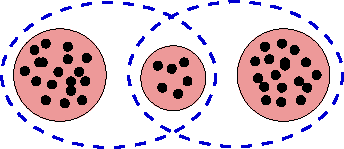
\includegraphics[height=17mm]{\figs/md-org}
    \end{columns}

    \begin{center}
      {\footnotesize
        \begin{tabular}{lccccc}
          ID & entity           & relation   & content & data storage & access control \\\hline
          \tt lfn & config      & mc         & yes     & yes  &  no            \\
          & $\downarrow$&            &         &      &  $\uparrow$    \\
          \tt \alert{mc}  & \alert{ensemble}    & ---        & yes     &  no  &  yes      \\
          & $\uparrow\uparrow\uparrow$ \\
          $*)$  & \color{blue}{publication} & set of mc  & yes     &  no            & no 
        \end{tabular}
      }
    \\[5mm]
    $*)$ ILDG 1.0 has no official registration of IDs or publication metadata yet!
    \end{center}
\end{frame}
%------------------------------------------------
\begin{frame}{DOI and Data Publishing}
  \begin{block}{Data Publishing}
    \begin{itemize}
    \item Registration of persistent identifier (DOI)
    \item Metadata for registration (DataCite)
    \item Landing Page (hosting and automatic generation)
    \item Harvesting of metadata
    \end{itemize}
  \end{block}

  Exploratory setups by \href{https://www.jldg.org/DOI}{JLDG} and
  \href{https://www.osti.gov/dataexplorer/search/product-type:Dataset/semantic:Lattice QCD}{USQCD}
  \begin{itemize}
  \item using national registration authorities (JaLC, OSTI)
  \item workflow and metadata for registration and generation of landing pages
  \end{itemize}

  Possible directions in ILDG 2.0
  \begin{itemize}
  \item establish workflow for registration, generation and hosting of landing pages
    (e.g. \href{https://zenodo.org/communities/ildg}{Zenodo})
  \item extended metadata support
  \item dedicated metadata harvesting (e.g. by INSPIRE)
  \item common registration authority
  \end{itemize}
  
\end{frame}
    
%------------------------------------------------
\begin{frame}{What does ``accessible'' mean?}
  \begin{alertblock}{Accessible}
    \begin{itemize}
      \item[A1~~] (M)D retrievable by ID using standardized protocols 
      \item[A1.1] protocol is open, free, and universally implementable 
      \item[A1.2] protocol allows authentication/authorization procedure where necessary 
      \item[A2~~] MD accessible even if data is no longer available
    \end{itemize}
  \end{alertblock}

  \begin{itemize}
  \item A1 can be achieved e.g. by a File Catalog: ID $\mapsto$ storage location(s)
  \item Accessible does not imply (unrealistic) public access without authentication
  \item MD is precious even without the associated data 
  \end{itemize}

  \vfill

\end{frame}
%------------------------------------------------
\begin{frame}{How does ILDG address ``accessible''?}
  \begin{center}
    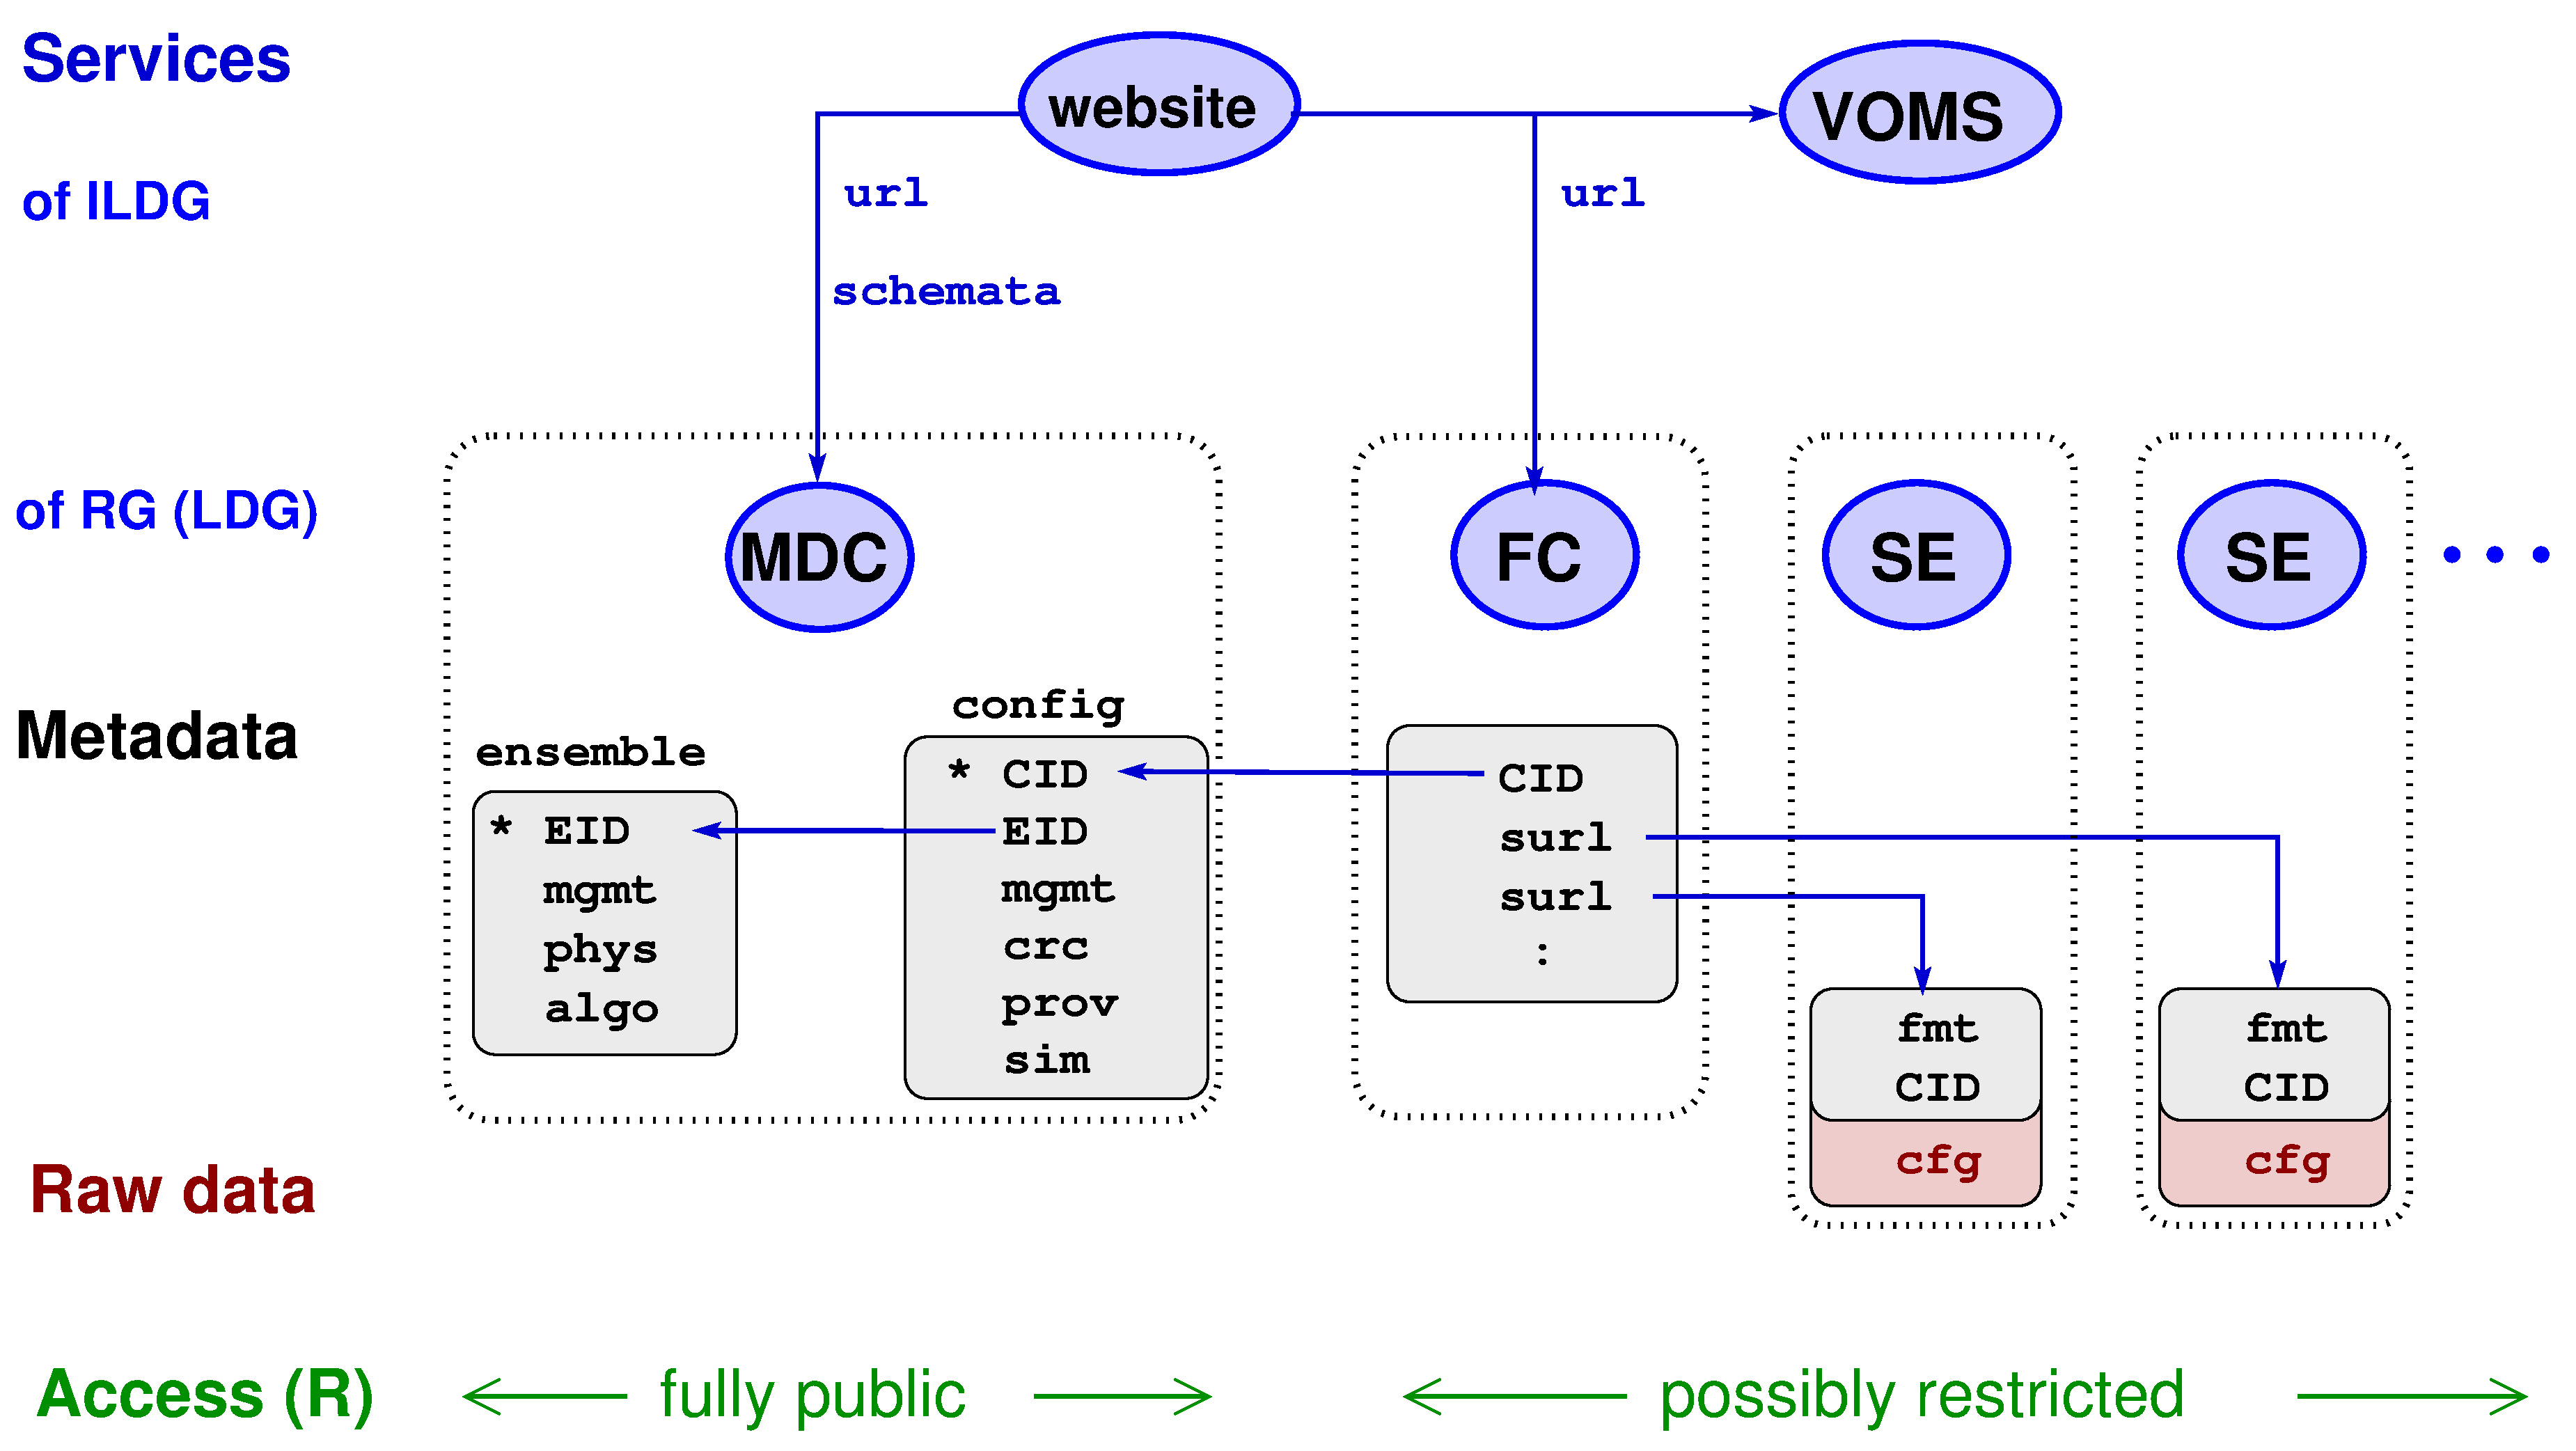
\includegraphics[height=40mm]{\figs/arch-ildg-db}
  \end{center}
  \begin{itemize}
  \item all metadata is \alert{publicly} accessible (from MDC)
  \item well-defined community-wide metadata \alert{schema}
  \item metadata available in a standard \alert{markup} language 
  \item standardized protocols and API of \alert{services} for access to data and metadata
  \end{itemize}
\end{frame}
%------------------------------------------------
\begin{frame}{What does ``interoperable'' mean?}
  \begin{alertblock}{Interoperable}
    \begin{itemize}
    \item[I1] (M)D use a formal, accessible, shared, and broadly applicable 
      language % for knowledge representation
    \item[I2] (M)D use vocabularies that follow FAIR principles
    \item[I3] (M)D include qualified references to other (M)D
    \end{itemize}
  \end{alertblock}

  \begin{itemize}
  \item ability of data (or tools) from non-cooperating resources\\
    to integrate (or work together) with minimal effort
    
  \end{itemize}
\end{frame}
%------------------------------------------------
\begin{frame}{How does ILDG address ``interoperable''?}

  \begin{block}{Common standards for}
    \begin{itemize}
    \item Metadata schema
    \item Data format
    \item API and URL for web services of regional grids
    \end{itemize}
  \end{block}

  New directions:
  \begin{itemize}
  \item Extend ILDG format to include support for \alert{HDF5}
    \begin{itemize}
    \item definition of ILDG packing rules
    \item convenient tools for packing and conversion
    \end{itemize}
  \item Token-based authentication
  \item REST API
  \end{itemize}
  
\end{frame}
%------------------------------------------------
\begin{frame}{What does ``reusable'' mean?}
  \begin{alertblock}{Reusable}
    \begin{itemize}
    \item[R1~~] (M)D richly described with plurality of accurate and relevant attributes
    \item[R1.1] (M)D released with clear and accessible data usage license
    \item[R1.2] (M)D associated with detailed provenance
    \item[R1.3] (M)D meet domain-relevant community standards
    \end{itemize}
  \end{alertblock}

  \begin{itemize}
  \item reference to a paper may not be sufficient
  \item good scientific practice $\leftrightarrow$ FAIR
  \item also related to verifiable invariance of results
    \hfill {\small \href{https://edbennett.github.io/uklft-talk-20220527/\#/2/1/4}{(see presentation by Ed Bennett)}}
    \begin{itemize}
    \item reproducibility: same data + same analysis
    \item replicability: new data + same analysis
    \item robustness: same data + new analysis
    \end{itemize}
  \end{itemize}

  \vfill

\end{frame}
%------------------------------------------------
\begin{frame}{How does ILDG address ``reusable''?}
  \begin{columns}[c] 
    \column{0.48\textwidth}
    {\bf Ensemble MD}
    \begin{itemize}
    \item Physics
    \item Algorithm
    \item Management
    \end{itemize}

    \vspace*{5mm}
    {\bf Config MD}
    \begin{itemize}
    \item Markov step
    \item Implementation (machine, code)
    \item Management (creator, date, checksum)
    \end{itemize}

    \vspace*{5mm}
    But \alert{no} license aspects! (cf. R1.1)

    \column{0.5\textwidth}
    \hspace*{-5mm}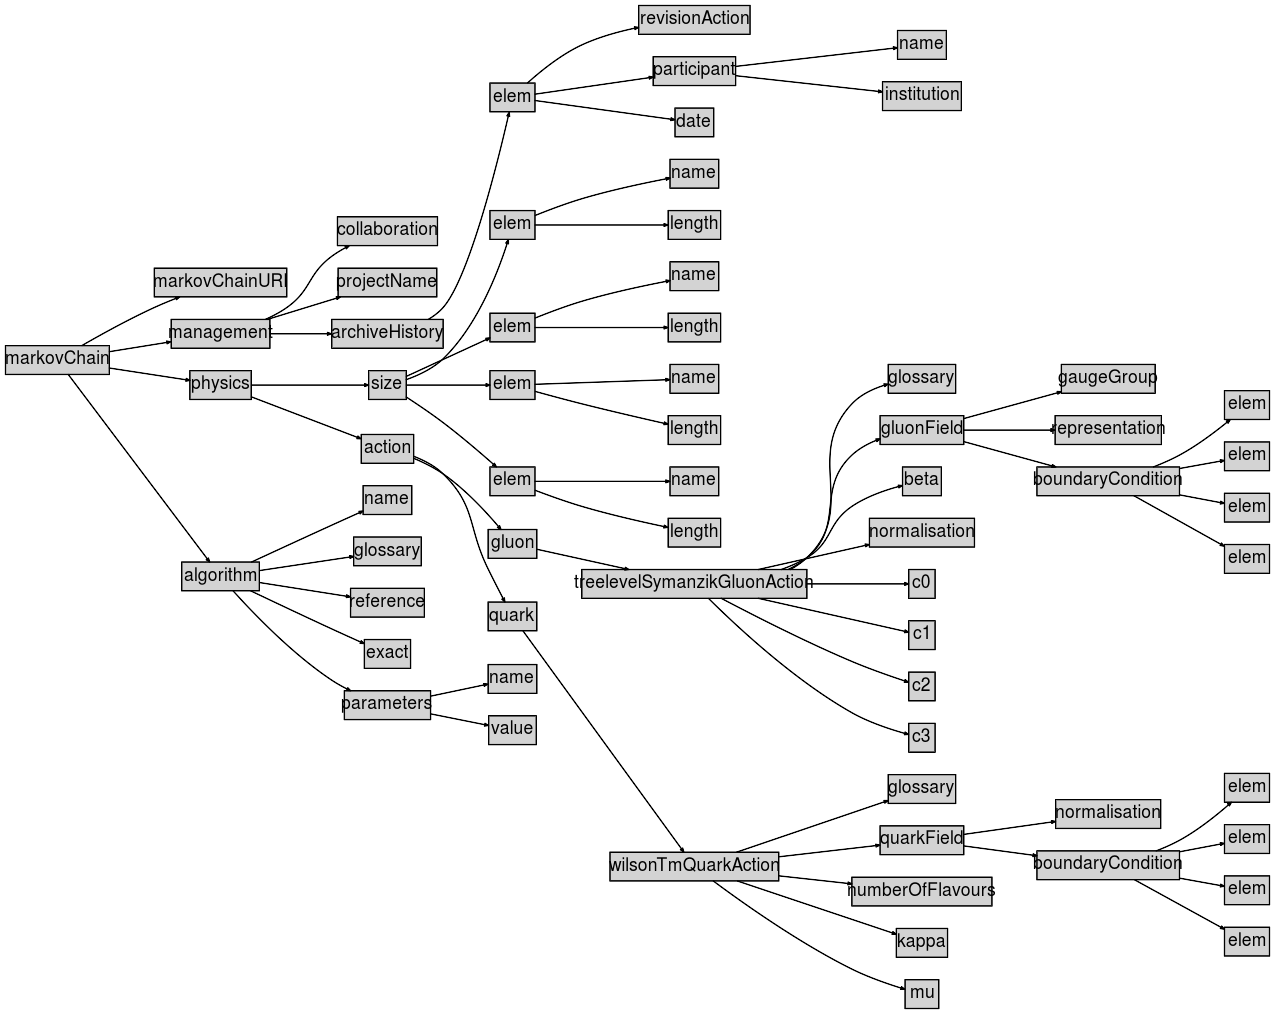
\includegraphics[height=65mm]{\figs/ensemble-tree}
  \end{columns}
\end{frame}

\end{document}


